\documentclass {article}
\usepackage{graphicx}
\usepackage{amsmath}
\renewcommand\vec{\mathbf}
\let\OldS\nabla
\renewcommand{\nabla}{\boldsymbol{\OldS}}

\let\OldHat\hat
\renewcommand{\hat}[1]{\OldHat{\mathbf{#1}}}


\begin{document}
\thispagestyle{empty}% empty header/footer

\begin{center}\strut
	\bfseries\Huge
	On Gravity and Radiation
\end{center}


\centerline{David Plotz}


\begin{center}\strut
March 10th, 2023
\end{center}
\vfill

	


\newpage

\section{Meta Theory}

Who, What, Where, When, Why, How?
\\[0.15in]
what?    A new theory of  gravity
\\
why?   100 years quantumgravity = GR + QM . Other proposals
\\[1in]


MVP - Beta Testing - Not ready for prime time
\\

What is a theory?
\\[1in]

Hypothesis vs. Postulate vs. Assumptions? (Main Hypothesis with mathematical framework postulates?)
\\[1in]



What does a theory of gravitation need?
\\[2in]

What would be nice to have? 
\begin{itemize}
	\item Simplicity : Occam's razor
	\item A wow!
\end{itemize}

\vspace{10pt}

Einstein asked Marcel Grossmann for help -- It's a big theory
\\[2in]

Structure: Lots of pre-amble to remind us: Maxwell's eqns, Solutions to Maxwell's eqns., including a stochastic version of it. The theory then begins in Massive particle, three results, and then the wow!

pet peeve:

scientific method and choice of hypothesis


\newpage


\section{Maxwell Equations}
\subsection{From Electromagnetism to Gravity-magnetism}



We assume that gravity is correctly described by Maxwell's Equations:

$$\nabla \times \vec B  - \partial_t \vec E  = -4 \pi G \vec J ~~~~~~~~ \nabla \times \vec E + \partial_t \vec B = 0    $$

$$\nabla \cdot \vec E = -4 \pi G \rho ~~~~~~~~~~ \nabla \cdot \vec B = 0   $$

and, for completeness, the conservation of mass-charge:

$$\nabla \cdot \vec J + \partial_t \rho = 0 $$

Where we are in units where c = 1. The constant G differs in different systems of units. In SI units, it is equal to $6.674 \times 10^{-11} \frac {N \cdot m^2}{kg^2}$ 

\newpage 
\subsection{Solenoidal and Irrotational Vectors}
While this step is not strictly necessary, and all of the results in the rest of the paper can still be derived, it actually tends to make the math a little cleaner to split the Maxwell equations into their Irrotational and Solenoidal forms.

A vector $\vec V$ can be split into a solenoidal vector $\vec V_S$ and an irrotational vector $\vec V_I$:

$$\vec V = \vec V_I + \vec V_S $$

where

$$\nabla \cdot \vec V_S = 0 ~~~~~ \nabla \times \vec V_I = 0 $$

Using this notation we can rewrite the Maxwell equations into irrotational equations:

$$\nabla \cdot \vec E_I = -4 \pi G  \rho$$

$$\nabla \cdot \vec J_I + \partial_t \rho = 0 $$

$$ \partial_t \vec E_I = 4 \pi G \vec J_I $$

And solenoidal equations:

$$\nabla \times \vec E_S + \partial_t \vec B_S = 0 $$

$$\nabla \times \vec B_S - \partial_t \vec E_S =  - 4 \pi G \vec J_S$$

The thing we really want to say, and I'm not sure if this is an assumption or is just totally obvious, is that, at least when we are in the rest frame of the mass (which is the frame of reference that we will be in for the rest of this paper), these equations de-couple. We have one set of equations that describe the forces due to the mass and another set of equations that describe radiation. We can make this explicit by defining a new current:

$$\vec {J_S'} = - G \vec {J_S}$$

which changes the inhomogenous Solenoidal equation into:

$$\nabla \times \vec B_S - \partial_t \vec E_S =  4 \pi \vec {J_S'} $$

but affects none of the other equations at all!

Because this form of the equations is the same as that presented in books on radiation. I will get rid of the prime on the Solenoidal current, and use the following equations as the solenoidal (radiation) Maxwell equations:

$$\nabla \times \vec B_S - \partial_t \vec E_S =  4 \pi \vec J_S$$

$$\nabla \times \vec E_S + \partial_t \vec B_S = 0 $$
\newpage

\section{Solutions to the Maxwell Equations}
\subsection{Spherical Vectors}
Following Berrara (http://iopscience.iop.org/article/10.1088/0143-0807/6/4/014/meta) we assume that any vector field, $\vec V$, and any scalar, $g$, can be expanded as follows:

$$\vec V (\vec x) = \sum_{l=0}^{\infty} \sum_{m=-l}^{l} \left[a_{lm}(r) \vec Y_{lm}(\theta, \phi) +b_{lm}(r) \left( \hat r \times \vec X_{lm} (\theta, \phi) \right) +c_{lm}(r) \vec X_{lm} (\theta, \phi) \right] $$

$$g(\vec x) = \sum_{l=0}^{\infty} \sum_{m=-l}^{l} g_{lm}(r) Y_{lm}(\theta, \phi)$$

where $Y_{lm}$ are the usual spherical harmonics (see Jackson 3.53), $\vec Y_{lm}$ is simply $\hat r Y_{lm}$  and $\vec X_{lm}$ is defined as,

$$\vec X_{lm}(\theta, \phi) = \frac {-i}{\sqrt{l(l+1)}} \vec r \times \left( \nabla Y_{lm}(\theta, \phi) \right) $$

The three vector spherical harmonics $(\vec Y_{lm}, \vec X_{lm}, \hat r \times \vec X_{lm} )$ obey a few relations compiled below for ease of reference:

$$\nabla  \cdot \left( f(r) \left( \hat r \times \vec X_{lm} \right) \right) = - i \sqrt {l(l+1)} \frac {f(r)} {r} Y_{lm}$$

$$\nabla \cdot \left( f(r) \vec X_{lm} \right) = 0 $$

$$ \nabla \cdot \left( f(r) \vec Y_{lm} \right) = \frac {1}{r^2} \frac d {dr} \left(r^2 f(r) \right) Y_{lm}$$

$$\nabla \times \left( f(r) \left( \hat r \times \vec X_{lm} \right) \right) = \frac {-1} {r} \frac d {dr} \left( r f(r) \right) \vec X_{lm}$$

$$\nabla \times \left( f(r) \vec X_{lm} \right) = \frac {i \sqrt{l(l+1)} } {r} f(r) \vec Y_{lm} + \frac 1 r \frac d {dr} \left( r f(r) \right) \left( \hat r \times \vec X_{lm} \right)$$

$$\nabla \times \left( f(r) \vec Y_{lm} \right) = \frac {- f(r)} r i \sqrt {l (l+1)} \vec X_{lm}$$

$$ \vec X_{lm} \cdot ( \hat r \times \vec X_{lm}) = \vec Y_{lm} \cdot  ( \hat r \times \vec X_{lm}) = \vec Y_{lm} \cdot \vec X_{lm} = 0$$ 

$$ \int \vec X_{lm} \cdot \vec X_{l' m'}^* ~ d \Omega  = \int \vec Y_{lm} \cdot \vec Y_{l' m'}^* ~ d \Omega  = \int ( \hat r \times \vec X_{lm}) \cdot ( \hat r \times \vec X_{l' m'}^*) ~ d \Omega  = \delta_{ll'} ~ \delta_{m m'} $$

$$\int \vec Y_{lm} \cdot \vec X_{l' m'}^* ~ d \Omega = \int \vec Y_{lm} \cdot ( \hat r \times \vec X_{l' m'}^* ) ~ d \Omega  =  \int \vec X_{lm} \cdot ( \hat r \times \vec X_{l' m'}^* ) ~ d \Omega   = 0 $$

\newpage
\subsection{Newton's gravity (Irrotational part of the Maxwell Equations)}

Skipping this sub-section is totally okay, but for completeness and as a way to introduce some notation, let's actually go ahead and derive that the gravitational field follows the inverse square law. 

For a static mass distribution, we have:

$$\rho = m \delta^3_x  $$

where I am purposefully being a little bit non-commital about the delta function. In this present paper, it doesn't matter so much, but I think it's best to leave it a little open for future work. With that said, we can still say that outside of some radius R, it looks like a pure delta function... i.e.,

$$\delta^3_x = \delta(\vec x) ~~~ \textrm{if} ~~~ r > R $$

Using the irrotational part of the Maxwell equations:

$$\nabla \cdot \vec{E}_I = -4 \pi G \rho ~~~~~~~~~~ \nabla \times \vec{E}_I = 0$$

and using the spherical vector harmonics we developed elsewhere (actually the section above in this version of the paper).  We first write $\vec E_I $ as follows:

$$\vec E_I =  \sum_{l,m} \left[a_{lm}\vec Y_{lm} +b_{lm} (\hat r \times \vec X_{lm}) +c_{lm}\vec X_{lm} \right] $$

We rewrite the curl equation (there's a better way to say this, but it's slipping my mind)

$$ 0 = \nabla \times \vec E_I  = \sum_{l, m} \left[ \left( - \frac 1 r \frac d {dr} (r b_{lm}) - i \sqrt {l ( l +1)}  \frac {a_{lm} } r \right) \vec X_{lm} + \frac {i \sqrt {l(l+1)} } r c_{lm} \vec Y_{lm} + \frac 1 r \frac d {dr} (r c_{lm}) (\hat r \times \vec X_{lm}) \right] $$

Thus,

$$ c_{lm} = 0 $$

and,

$$a_{lm} = - \frac i {\sqrt{l(l+1)} }\frac d {dr} (r b_{lm}) $$

The divergence of $\vec E_I$ gives,

$$ 4 \pi G \sum_{l, m} \rho_{lm} Y_{lm} = \sum_{l, m} \left[ \frac 1 {r^2} \frac d {dr} (r^2 a_{lm} ) - i \sqrt{l(l+1)} \frac {b_{lm}} r  \right] ~ Y_{lm} $$

Using this equation with our solution for $a_{lm}$ and setting 

$$B_{lm} = i \frac {r ~ b_{lm}} {\sqrt {l (l+1)}} $$

We have

$$\frac 1 {r^2} \frac d {dr} \left( r^2 \frac d {dr} B_{lm} \right) - \frac {l(l+1)} {r^2} B_{lm} = 4 \pi G \rho_{lm}$$

The solution to this is well-known (see Jackson). We define,

$$q_{lm} \equiv \int Y_{lm}^* (\theta, \phi) r^l  \rho (\vec x) ~ d^3x = \int \rho_{lm} (r) r^{l+2} ~ dr $$

Then 

$$ B_{lm} = - \frac {4 \pi G \rho_{lm}} {(2l +1) r^{l+1}} $$ 
 

And we can write out the final solution:

$$\vec E_I(\vec x) = \sum_{l,m} \left[ -\frac {4\pi i G }{2l+1} \frac {q_{lm}}{r^{l+2}} \sqrt {l(l+1)} \left(\hat r \times \vec X_{lm} \right)  - \frac {4 \pi G (l+1)}{2l+1} \frac {q_{lm}}{r^{l+2}} \vec Y_{lm} \right] $$


Clearly then, if

$$\rho = m\delta(\vec x) $$

We get

$$\vec E_I(\vec x) = - \frac {mG} {r^2}  ~~~~~~~~~~~ \textrm{if} ~~~ r > R$$

as expected.
\newpage
\subsection{Radiation (Solenoidal part of the Maxwell Equations)}

In the previous section we looked at the Irrotational part of the Maxwell Equations when there was no current.

Now we will look at the solenoidal part of the Maxwell Equations:

$$\nabla \times \vec E_S + \partial_t \vec B_S = 0 $$

$$\nabla \times \vec B_S - \partial_t \vec E_S =  - 4 \pi G \vec J_S$$

In a region of empty space, i.e., everywhere outside of the radius $a$ of our model of a massive particle (please see the section on the model of a Massive particle). We are left with 

$$\nabla \times \vec E_S + \partial_t \vec B_S = 0 $$

$$\nabla \times \vec B_S - \partial_t \vec E_S =  0$$

These will set-up the well-known wave equations. Assuming a time dependence $e^{-iwt}$, in spherical coordinates, the general solution is

$$\vec B_S (\vec x) = \sum_{l, m} \left[ a_E(l,m)f_l(kr) \vec X_{lm}(\theta , \phi) - \frac i k a_M (l, m) \nabla \times \left(  g_l (kr) \vec X_{lm} (\theta , \phi) \right) \right]$$

$$ \vec E_S (\vec x) = \sum_{l, m} \left[ \frac i k a_E(l,m) \nabla \times  \left( f_l (kr) \vec X_{lm}(\theta, \phi)\right) + a_M(l,m) g_l (kr) \vec X_{lm}(\theta, \phi) \right]$$

The functions $f_l$ and $g_l$ are linear superpositions of the radial Hankel functions,

$$h_l^{(1)}(x) = -i (-x)^l \left(\frac 1 x \frac d {dx} \right)^l \left(\frac {e^{ix}} x \right)$$

$$h_l^{(2)}(x) = \left( h_l^{(1)}(x) \right)^*$$

\noindent $a_E$ and $a_M$ as well as the particular dependence of $f_l$ and $g_l$ on $h_l^{(1)}(x) $ and $h_l^{(2)}(x) $ depend on the boundary conditions.

In our case, we are looking at a massive particle that sinks radiation, we therefore need to only include incoming waves.

The total instantaneous power radiated (perhaps we should say sunk) is defined as.

$$P \equiv \int_V d^3x ~ \nabla \cdot \left( \frac 1 {8 \pi} \vec E \times \vec B^*\right) = \oint_{\partial V} \hat r \cdot \vec S ~ da = R^2 \int d\Omega ~ \hat r \cdot \vec S \bigg|_{r = R}$$

Using the relationships in the introduction on Vector Spherical harmonics, we find that we are left with only two non-vanishing terms,

$$P = \frac {R^2}{8 \pi} \sum_{l, m} \left[  \frac {-i} k |a_E|^2 h_l^{(2)} \frac 1 r \frac d {dr} \left( rh_l^{(1)} \right) + \frac i k |a_M|^2 h_l^{(1)} \frac 1 r \frac d {dr} \left( rh_l^{(2)}\right) \right]_{r=R}$$

Since, by assumption (I realize I never spelled this out elsewhere) the massive particle is electromagnetically neutral on average, we need neither the Transverse Magnetic nor the Transverse Electric modes to dominate. Thus, the two proportionality terms must obey $|a_E|^2 = |a_M|^2$. Use of the Wronskian leaves a particularly simple form for the power radiated,

$$P = \sum_{l,m} \frac {|a_E|^2} { 4 \pi k^2}$$

It also may be useful to derive the energy in this field. We can use the lowest order approximation, where we keep only terms of order $1/r$. In this approximation, the radiation fields behave like

$$\vec B (\vec x) \approx \sum_{l,m} \left[ a_E (l,m) f_l (kr) \vec X_{lm} (\theta, \phi) + a_M (l, m) g_l (kr) \left( \hat r \times \vec X_{lm} (\theta, \phi)  \right) \right]$$

$$ \vec E \approx - \hat r \times \vec B(\vec x) $$

We expect, after averaging over the noise (see the section on S.E.D.), 

$$|f_l|^2 = |g_l|^2 =  \frac 1 {k^2 r^2}$$

The energy in a spherical shell at $r =R$ is then (reading this now ... so many years later ... I think there's a different way of saying this... see Jackson 9.135)

$$\frac {dU} {dr} \bigg|_{r=R} = \frac 1 {16 \pi} \int \left( |\vec E  |^2 + |\vec B |^2 \right) r^2 ~ d\Omega  \bigg|_{r=R} = \sum_{l, m} \frac 1 {8 \pi} \frac {|a_E|^2}{k^2}$$

The momentum of the field in the volume $V$ is

$$\vec P_{\text{field}} = \frac 1 {8 \pi} \int_V \vec E \times \vec B^* ~ d^3x$$ 

$$\vec P_{\text{field}} = - \hat r \sum_{l, m}   \int_V \frac 1 {4 \pi}  \frac {|a_E|^2 |\vec X_{lm} |^2}{k^2 r^2} ~ d^3x $$

All that is left is to use the boundary conditions to determine $|a_E|^2$. This will be done in the subsection: Collapse and Stability


\newpage

\section{Stochastic Electrodynamics}
\subsection{Stochastic Electrodynamics}
I feel like there are probably a few good ways to introduce this topic. However, I think motivating it with pure observed fact is probably good.

Recently, maybe 20 years ago now, it was discovered that the universe is bathed in thermal radiation. This radiation is called the Cosmic Microwave Background Radiation. 

This thermal bath displays the black-body radiation distribution

$$\rho(w, T) = \frac {w^2} {\hbar^2} \left( \frac{ \hbar w}{e^{\hbar w / k_B T} - 1} + \frac 1 2 \hbar w    \right)$$

For our discussions, the most important this to consider is when $T \rightarrow 0$ and we are left with only the "zero-point" term $\hbar w / 2$. In quantum mechanics, this term is usually seen as a curious blemish that is generally removed across the board. Classically, this term has been studied by T.H. Boyer, with continued research by several others.

Researchers using the classical approach developed by T.H. Boyer, which I will briefly outline below, have found a remarkable number of exact agreements with quantum mechanics including "the retarded van der Waals force, ground state distribution of harmonic oscillators, Landau diamagnetism, Planck spectrum of blackbody radiation, and Debye specific-heat law for solids. Recently, it was further shown that parametric interaction can give rise to discrete SED excitation spectra that are in excellent agreement with QM predictions" - Huand and BAtelaan. 

The basic idea of Stochastic Electrodynamics (SED) is that the universe is bathed in a random thermal bath with a particular energy density. The random characteristics of this thermal bath are most easily understood by adding in a Gaussian noise term $W$ with the following properties:

$$<W> = 0$$
$$<W_i (\vec k) W_j (\vec k') > = \delta_{ij} \delta^3(\vec k - \vec k')$$

In Cartesian free space, we have:

$$\vec E (\vec x ,  t) = \text {Re} \sum_{\lambda = 1}^2  \int d^3k ~ \hat \epsilon(\vec k, \lambda) \sqrt {\frac {\hbar w} {2 \pi^2}} W_{\lambda}(\vec k) \exp(iwt - i\vec k \cdot \vec x)$$

$$\vec B (\vec x ,  t) = \text {Re} \sum_{\lambda = 1}^2  \int d^3k ~ \frac {\vec k \times \hat \epsilon(\vec k, \lambda)} k \sqrt {\frac {\hbar w} {2 \pi^2}} W_{\lambda}(\vec k) \exp(iwt - i\vec k \cdot \vec x)$$


Boyer has shown that these equations lead to the correct spectral energy density for blackbody radiation as well as being Lorentz invariant.




\newpage

\section{Massive Particle}
\subsection{Main Hypothesis}

We also must talk about the temperature of the mass, it should be a perfect absorber at this basic level of the theory. And it absorbs all frequencies of radiation up to a cutoff.  Hopefully future researchers can dig into this and higher order approximations.

From the section on Radiation, we have:

$$\vec P_{\text{field}} = \frac 1 {8 \pi} \int_V \vec E \times \vec B^* ~ d^3x$$ 

$$\vec P_{\text{field}} = - \hat r \sum_{l, m}   \int_V \frac 1 {4 \pi}  \frac {|a_E|^2 |\vec X_{lm} |^2}{k^2 r^2} ~ d^3x $$


Taking the constants together, we rewrite this as 

$$\vec P  = - \hat r  \frac {\alpha}{r^2} $$

We will that the constant that satisfies the boundary conditions (conservation of energy, as shown in the next section), leads us to 

$$\vec p = - \hat r \frac {Gm \hbar} {r^2} $$


Which leads us to our main hypothesis:  Mass sinks radiation, with the following formula :

$$\boxed{ \vec p = - \hat r \frac {Gm \hbar} {r^2} } $$

This is our hypothesis, so for the remainder of the paper we can assume that this is true?

a little philosophy aside. Is this a force? Well, not really, because $F = m \cdot a$, and light doesn't have a mass, nor can it be accelerated. So what mechanism is causing this? Is it, in the quantum mechanical realm, caused by an interaction between the graviton and photons? I hope future researchers will look into this, but for this paper, I believe I can set a hypothesis, and then we just follow the math, and see what comes out of it.

\vspace{10pt}

There is a furhter step that we must take. Just as we assume a smallest radius for the mass (see the next section on the model of a massive particle), we must also assume a highest frequency that the mass is able to sink (this should be testable). Using the same arguments above, based on energy considerations, I will state that the maximum frequency supported by a mass follows from the same energy equation:

$$U = m = \hbar w = \hbar \int_0^w ~dw'$$

\noindent and therefore, the maximum $w$ is simply $m / \hbar$

I should probably make a table similar to the one in the next section dealing with radii and various real sources, but I think for now it suffices to say that $m / \hbar $ is generally a very, very big number.



\newpage
\subsection{Model}
The following long quote is from Rohrlich because I don't know how to say it any better than he did. It has been modified from the original to reflect that we are talking about massive particles and not charged particles.

We wish to construct a model of a massive particle. ``The most obvious model of a massive particle is a sphere carrying a spherically symmetrical mass distribution. While such a model is meant (and was indeed proposed) as a picture of a massive elementary particle (a neutron, for example), it is obvious that is is basically a macroscopic massive body, only much smaller. There is nothing 'elementary' about it. To see this clearly, let us consided a macroscopic massive sphere in more detail.

``Consider a sphere of radius $R$ and spherically symmetric mass density $\rho (\vec x)$. Its total mass is

$$ m = \int_V \rho(\vec x) d^3x$$

``The integral extending over the volume of the sphere. Since $m \neq 0$ by assumption, there must exist attractive gravitational forces between 'parts' of the total mass. Symmetry would therefore require that this massive sphere contract and continue to do so to arbitrarily small radius $R$." Thus with no other forces present, the particle will necessaruly collapse.

In the next section, I will show that the particle need not collapse. For now, however, let us take it as an assumption that the particle does not collapse. Since we are assuming that there are no other forces in play besides for the gravitational one, its total energy must be

$$U = m = - \frac 1 2 \int \frac {Gm \rho(\vec x)} {r} d^3x$$

We also must notice the negative energy, and in fact take 

$$U^2 = m^2$$

To complete the computation, we must choose some mass density distribution to integrate over. Mathematically, the simplest is a uniform spherical shell at the radius $R$, in which case

$$m = \frac {Gm^2} { 2R} ~~~~~ or  ~~~~ R = \frac {Gm} 2 $$

If, however, we choose a different mass density distribution (a uniform sphere for example), we find that the radius $R$ will always be of the order $Gm$. Therefore, I have chosen $R = Gm$ as the mathematical limit of the radius of a massive particle. This radius is similar in spirit to the classical radius of an electron.

It is useful to compare the mathematical radius with the radii of real physical bodies. Slipping back to SI units, we give a short list of real macroscopice objects with $\Phi = \frac {Gm}{Rc^2}$

$$\text{Mathematical limit:  } ~~~ \Phi = 1 = \frac {Gm}{Rc^2}$$
$$\text{Black hole:  } ~~~ \Phi = 1$$
$$\text{Sun:  } ~~~ \Phi = 2 \times 10^{-6}$$
$$\text{Earth:  } ~~~ \Phi = 7 \times 10^{-10}$$
$$\text{Proton:  } ~~~ \Phi = 1\times 10^{-38}$$


\newpage
\subsection{Conservation of Energy - Collapse and Stability}

$$U = \frac 1 {16 \pi} \int \left( |\vec E  |^2 + |\vec B |^2 \right) ~ d^3x $$

The energy of the field in the volume $V$ is


$$U  =\sum_{l, m}   \int_V \frac 1 {4 \pi}  \frac {|a_E|^2 |\vec X_{lm} |^2}{k^2 r^2} ~ d^3x $$

The energy density can thus be defined as

$$u  = \sum_{l, m}   \frac 1 {4\pi}  \frac {|a_E|^2 |\vec X_{lm} |^2}{k^2 r^2} $$

Taking the constants together, we rewrite this as 

$$u  =  \frac {\alpha}{r^2} $$


Mysteriously, we now take the integral over $w$ with the cutoff at $m/ \hbar$

$$u = \int_0^{m/ \hbar}  \frac {\alpha}{r^2} ~dw = \frac {\alpha m}{\hbar r^2}$$

Our goal is to now find $alpha$


We will show that there is conservation of energy, and therefor the massive particle introduced in the last section will not collapse (One could have also done this purely from a pressure standpoint, but Energy conservation seems cooler)

$$U = \int_V u ~ d^3x = \int_V \left( - \frac 1 G |\vec E_I |^2  +  |\vec E_S |^2  +  |\vec B_S |^2 \right) ~ d^3x$$

$$U = - \frac {Gm^2} R + \frac {4 \pi \alpha m R} \hbar$$

If this is a constant, then energy is conserved. More to the point, if we say these two energies cancel each other out, then we are left with zero energy, thus we can write

$$\alpha = \frac 1 {4 \pi R^2} Gm \hbar$$

and thus 

$$u  = \sum_{l, m}   \frac 1 {4\pi}  \frac {|a_E|^2 |\vec X_{lm} |^2}{k^2 r^2}  =  \frac 1 {4 \pi R^2} \frac {Gm \hbar} {r^2} $$

A similar treatment for pressure would have left us with 

$$p = - \hat r \frac 1 {4 \pi R^2} \frac {Gm \hbar} {r^2} $$

Possibly with some factors of $2 \pi$

Now we come to the crazy bug in the theory. What we want to do is use something we have learned from Fourier transforms:

$$\psi (x) = \int \psi(k)e^{-ikx} ~ dk $$

$$\psi ( k ) = \frac 1 {2 \pi} \int \psi(x) e ^{ikx} ~ dx $$

Which we combine to write

$$\psi(x) = \frac 1 {2 \pi} \int \int \psi (x') e^{ik(x' - x)} ~dk ~dx'$$


And here is our bug, if we set $k$ = $1/R$ (which is totally not plausible), then, besides for some factors of  $\pi$, we have

$$U =\frac 1 {8 \pi^3} \int \int \frac {Gm\hbar}{r^2} ~d^3x ~ d^3k$$

and 

$$\vec P = -\frac {\hat r} {8 \pi^3} \int \int \frac {Gm\hbar}{r^2} ~d^3x ~ d^3k$$
 

\newpage


\subsection {Conservation of Momentum and Ohm's Law}

Here and in everything that follows, as per usual when talking about radiation, it's easier to stay in k-space.

Conservation of momentum requires

$$\int_V \left(  \rho \vec E_I  + \vec J_S \times \vec B_S \right) ~ d^3x  = 0 $$

(See Jackson 6.114)
\\
\\

Ohm's law states that the current is proportional to the electric field:

$$\vec J_S = \sigma \vec E_S$$ 

Assuming harmonic time dependency $e^{-iwt}$ we have

$$- \hat r \int_V \left(  m \delta (\vec x) \frac {Gm}{r^2}  - \sigma \frac {Gm \hbar} {r^2} \right) ~ d^3x  = 0 $$

Therefore,

$$\sigma = \frac m \hbar \delta (\vec x) $$

Note, there may be a factor of $4 \pi $ missing (clean up will happen at some other time):

$$\sigma = \frac m {4 \pi \hbar} \delta (\vec x) $$


\newpage

\section{Three classical Experiments}
\subsection{Precession of the perehilion of Mercury}


Coulomb's law is only true for static fields. For moving masses, we must perform a Lorentz boost. If we perform a  Lorentz boost from the frame of a charged particle to a different frame moving at a velocity $\vec v$, we get the transformed fields:

$$\vec E' = \gamma \vec E - \frac {\gamma^2} {\gamma + 1} \vec v (\vec v \cdot \vec E) $$

$$ \vec B' = - \gamma \vec v \times \vec E$$

where 

$$ \gamma = \frac 1 {\sqrt{1 - \vec v^ 2} } $$ 

We therefore see that the reason that electrostatics works under a Lorentz transformation is that we introduce a new field into the equations called the "magnetic" field.

In our everyday experiences, it seems clear that there is no "gravitational magnetic" field. However, just as we have learned from special relativity, our observations are limited because we do not travel at speeds where the Lorentz transformation becomes noticeable. Similarly, we live on the Earth and to our observations it does not move. Therefore we have become accustomed to only thinking about "stationary" gravity, i.e., gravity from a large mass that is considered to be unmoving in that frame of reference. With this in mind, let us assume that there is a "gravitational magnetic" field and see what effect it would have.

We define the gravitational field $\vec E_g $ as

$$ \vec E_g = \vec F / m $$

where $F$ is the gravitational force, and $m$ is a test mass. Thus we define the gravitational field of a massive object at the origin acting on a sall test-body at a distance $r$ away from the origin ag

$$\vec E_g = - \frac {Gm} {r^3} \vec r $$

We then perform a Lorentz-transformation to a new frame moving at some velocity $\vec v$. By assumption, we use the same Lorentz transformaation as before:

$$\vec E_g' = \gamma \vec E_g - \frac {\gamma^2} {\gamma + 1} \vec v (\vec v \cdot \vec E_g) $$

$$ \vec B_g' = - \gamma \vec v \times \vec E_g$$

Thus, if the Lorentz transformation is to apply to Newtonian gravity, we must introduce this "gravitational magnetic" field. Is this magnetic field observable? The answer is yes.

We wish to examine what is known as  Kepler's problem. When two objects are in orbit around each other, see the figure below, we expect from classical Newtonian mechanics:

$$ U_{\text{Newt}} = \frac m 2 (\frac {dr} {dt})^2 - \frac {GMm} r + \frac {l^2} {2mr^2}$$

where $l^2 = m^2 (\vec r \times \vec v)^2$

\begin{center}
	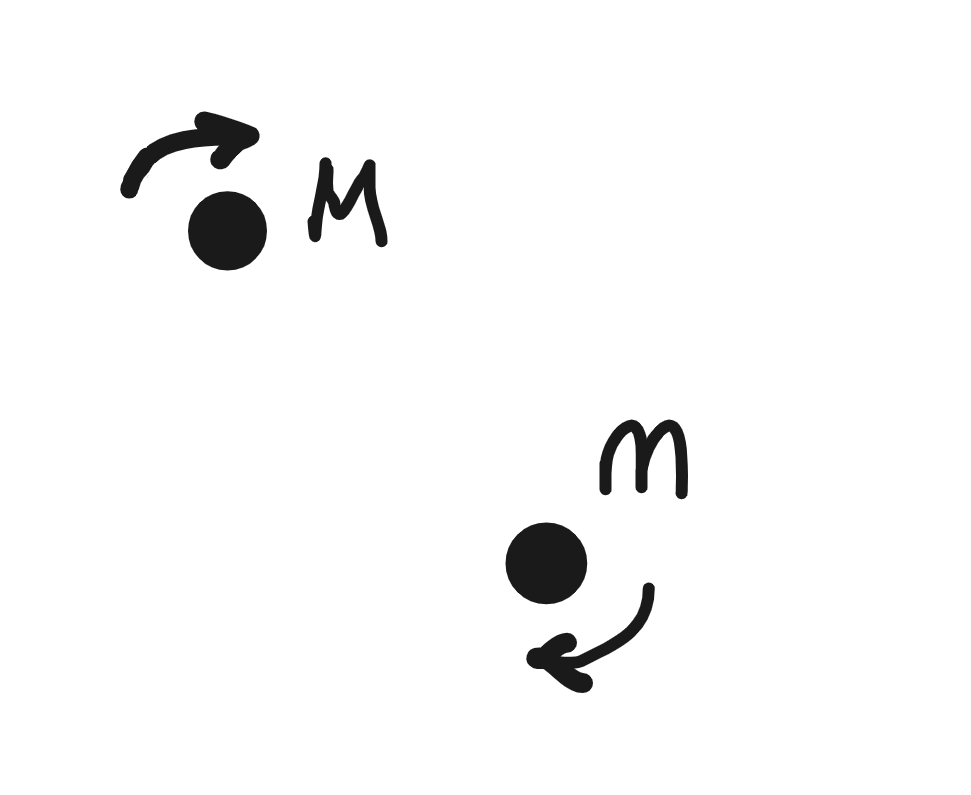
\includegraphics[scale=0.1]{autodraw.png}
\end{center}

Now, it is well known that when an electron moves it induces a magnetic moment, defined as:

$$\vec m_{moment} \equiv \frac 1 {2} e (\vec r \times vec v)$$

So, using our assumption that we simply transform electric charge to mass, we will simply replace $e$ with $m$, and assume that when a mass moves, there is a corresponding "gravitational magnetic moment":

$$\vec m_{gravitational moment} \equiv \frac 1 {2} m (\vec r \times vec v)$$

Adding in the magnetic interaction is straightforward in the low velocity limie, i.e., wehen $v << 1$. Our transformed fields will then be

$$\vec E_g' = \vec E_g$$

$$ \vec B_g' = - \vec v \times \vec E_g$$

Thus in the low velocity limit:

$$\vec B_g = - \vec v \times \vec r \frac {GM} {r^3} $$ 

The potential energy $U$ of a magnetic moment in an external field is given by:

$$U = - \vec m \cdot \vec B = \frac 1 2 m (\vec r \times \vec v)\left(\vec v \times \vec r \frac {GM} {r^3} \right) = - \frac {GMm} 2 (\vec r \times \vec v)^2$$

A similar contribution is given to the potential energy of the system when viewed from the other mass, thus doubling the above. 

Thus, with the addition of the gravitational magnetic field , the solution to Kepler's problem is modified by this additonal term:

$$ U_{\text{Einstein}} = \frac m 2 (\frac {dr} {dt})^2 - \frac {GMm} r + \frac {l^2} {2mr^2} - \frac {GMl^2}{mr^3}$$

This is the same equation that one can achieve with General Relativity. 

According to Carroll: "A similar analysis of orbits in Newtonian gravity would have produced a similar result; the general equation (5.65) would have been the same, but the effective potential (5.66) would not have had the last term. (Note that this equation is not a power series in $1/r$, it is exact.)"

The important point to note, is that in this current theory presented in this paper. This is not exact, but is only the first order approximation. Further mathematical sophistication should lead to range of tests that could be performed to see which is the true theory of nature.


\newpage
\subsection{Bending of light around a mass}
This section concerns the two classical test of General Relativity concerning the bending of light around a massive object and the blue-shift of light as it falls down towards a massive object.

Main Postulate / Hypothesis: Empty space is filled with a randomly-fluctuating zero-point energy and a massive object absorbs some of this energy, thereby preventing collapse of the mass. I therefore postulate that a massive object induces a “field” (or maybe a momentum-flow is a better way to say it? sink?) in the surrounding space and when a photon travels through this “field,” the momentum of the photon is shifted in an additive and linear manner – in accordance with the following equation: 

$$\Delta \vec p = \int_{path} \vec P ~ dl ~~~~~~~~~~~ (30)$$

where we integrate along the path of the photon and $\vec P$ is defined as

$$\vec P = - \hat r \frac {Gm\hbar}{r^2} ~~~~~~~~~~~ (31)$$

We imagine a photon that emanates from a distant source, passes close by a massive object, then continues beyond the object to an observer. The closest point while passing, i.e., the impact parameter, is at a distance of $b$ from the center of the object. For ease of calculation, we will say that both the point of emanation and the observer are infinitely far from the massive object.

\begin{center}
	\includegraphics[scale=0.4]{light-bending.png}
\end{center}


We assume that to a first-order approximation the trajectory of the photon is a straight line. To calculate its change in momentum, we integrate along the straight-line path of the photon:

$$\Delta \vec p = \int_{path} \vec P ~ dl = \int_{-\infty}^{\infty} - \frac {Gm\hbar}{r^3} \vec r ~ wdz $$

We divide the problem into two parts: the momentum change in the direction parallel to the direction of travel of the photon and the momentum change perpendicular to the direction of travel. In calculating the momentum change in the direction parallel to the direction of travel, we note that as the photon approaches and then recedes from the massive object, the change in momentum cancels out to leave zero net change in the parallel direction. We can easily calculate the change in momentum in the direction perpendicular to the direction of travel:

$$\Delta p_y = \int_{-\infty}^{\infty}  \frac {Gm\hbar}{(z^2 + b^2)^{3/2}} b ~ wdz $$

This yields:

$$\Delta p_y = \hbar w \frac {2Gm} b$$

We therefore get:

$$\theta \approx \sin \theta = \frac {\Delta p_y}{p_z} = \frac {2Gm} b$$

Which yields the deflection angle:

$$\alpha = \frac {4Gm} b$$

This is the same result as in the theory of General Relativity.

\newpage
\subsection{Light falling in a gravity well}

Using the same postulate, we can calculate the blue-shift of light. As a photon falls into a gravity well, the momentum and hence the energy of the photon are shifted. Because the energy of a photon is generally expressed as a frequency, we say that the frequency of the photon observed at infinity is changed compared to when it is observed in a gravitational field at a distance R from the center of the massive object. We use the following equation to express this change:

$$\hbar w' = \hbar w + \Delta p $$

To calculate the change in momentum, we again integrate along the path of the photon:

$$\Delta p = \int_{\infty}^R \hat r \cdot \vec P w dr= \int_{\infty}^R - \frac {Gm\hbar}{r^2} w dr = \hbar w \frac {Gm}R $$

This yields:

$$\hbar w' = \hbar w \left( 1 + \frac {Gm}R \right) $$

At lowest order approximation, this is the same as that found in General Relativity

\newpage

\section{The Wow!}
\subsection{Dual transform}

The dual transform is carefully explained in Jackson in section 6.11: On the question of Magnetic Monopoles.

For now, we drop the subscript of Irrotational and Solenoidal, because it will be easier to work with. Here's Jackson:

``Let us suppose that there exist magnetic charge and current densities, $\rho_m$ and $\vec J_m$, in addition  to the electric densities, $\rho_e$ and $\vec J_e$, The Maxwell equations would then be

$$\nabla \times \vec B  - \partial_t \vec E  = \vec J_e  ~~~~~~~~ \nabla \times \vec E + \partial_t \vec B =  - \vec J_m   $$

$$\nabla \cdot \vec E = \rho_e ~~~~~~~~~~ \nabla \cdot \vec B =  \rho_m $$

``The magnetic densities are assumed to satisfy the same form of the continuity equation as the electric densities. It appears from these equations that the existence of magnetic charge and current would have observable electromagnetic consequences. Consider, however, the following \textit{duality trnsformation}:

$$\vec E = \vec E' \text{cos } \xi + \vec B'  \text{sin } \xi$$

$$\vec B = \vec B' \text{cos } \xi - \vec E'  \text{sin } \xi$$

$$\rho_e = \rho_e'  \text{cos } \xi  + \rho_m'  \text{sin} \xi  ~~~~~~~~~~ \rho_m = \rho_m'  \text{cos } \xi  - \rho_e'  \text{sin} \xi $$

$$\vec J_e = \vec J_e' \text{cos } \xi + \vec J_m' \text{sin } \xi ~~~~~~~~~ \vec J_m = \vec J_m' \text{cos } \xi  - \vec J_e' \text{sin } \xi $$

\noindent then it is straightforward algebra to show that the generalized Maxwell equations are invariant.

``The invariance of the equations of electrodynamics under duality transformations shows that it is a matter of convention to speak of a particle possessing an electric charge, but not a magnetic charge. The only meaningful question is whether \textit{all} particles have the same ratio of magnetic to electric charge. If they do, then we can make a duality transformation, choosing the angle $\xi$ so that $\rho_m = 0, ~ \vec J_m = 0$. We then have the Maxwell equations as they are usually known.

\newpage

\subsection{Spinor Transformation}

We note that we can write:

$$\nabla \times \vec V = g_i \partial_i \vec V $$

where the $g_i$s are defined:

$$g_1 = \left(\begin{matrix}  0 && 0 && 0 \\ 0 && 0 && -1 \\ 0 && 1 && 0 \end{matrix}\right) $$

$$g_2 = \left(\begin{matrix}  0 && 0 && 1 \\ 0 && 0 && 0 \\ -1 && 0 && 0 \end{matrix}\right) $$

$$g_3 = \left(\begin{matrix}  0 && -1 && 0 \\ 1 && 0 && 0 \\ 0 && 0 && 0 \end{matrix}\right) $$


We  define 

$$\gamma^0 = \left(\begin{matrix}  -1 && 0 \\ 0 && -1 \end{matrix}\right)$$

$$\gamma^i = \left(\begin{matrix}  0 && g_i \\ -g_i && 0 \end{matrix}\right)$$

There's actually some literature on spinors, and transforming from different representational spaces, but I'm not sure how useful it is. If it turns out useful, I know a book that goes over it carefully. 

\newpage

\subsection{Dirac Equation}



Using the equations we got for the current in the section on conservation of momentum, we can re-write the Maxwell equation dealing with current:

$$\nabla \times \vec B_S  - \partial_t \vec E_S  = - \frac m {\hbar} \vec E_S ~~ \delta^3_x$$

If we promise to only work "On shell", i.e., where we are on the shell of the mass, see the section concerning our model, we can therefore write this as

$$\nabla \times \vec B_S  - \partial_t \vec E_S  = - \frac m {\hbar} \vec E_S $$

Using the dual transform, see the section up above, we can re-write the two Solenoidal equations:

$$-\partial_t \vec E_S + \nabla \times \vec B_S   +\frac m {\hbar} \vec E_S = 0 $$ 

$$ -\partial_t \vec B_S - \nabla \times \vec E_S   +\frac m {\hbar} \vec B_S = 0$$ 


Using the transformation in the spinor section, we  re-write Maxwell's equations as 

$$-\partial_t \vec E_S + g_i \partial_i \vec B_S   +\frac m {\hbar} \vec E_S = 0 $$ 

$$ -\partial_t \vec B_S - g_i \partial_i \vec E_S   +\frac m {\hbar} \vec B_S = 0 $$ 


if we the define 

$$\psi = \left(\begin{matrix}  \vec E_S \\ \vec B_S \end{matrix}\right) $$

and use the other spinors we wrote in the previous section, we can again re-write Maxwell's equations as

$$\left(\gamma^{\mu} \partial_{\mu} + \frac m {\hbar} \right) \psi = 0 $$

which can be compared with, for example, Sakurai's book "Advanced Quantum Mechanics" equation 3.31.

\newpage

\section{Meta Theory 2}
In conclusion, we didn't set out to make quantum gravity ... but what we got was a set of equations that unified gravity, electromagnetism and quantum mechanics.

From Zwiebach: "Over the course of time, the development of physics has been marked by unifications: events when different phenomena were recognized to be related..."


See the forest for the trees -- Yeah, there may be a rotten tree here or there, but the forest is healthy.
\newpage


\end{document}
